\newpage
\subsubsection{Stomach Cancer Data}
We apply the APC2- and LCC-models to the stomach cancer data set and analyse the prediction results in the same manner as for the lung cancer data. Overall, we observe that the two models perform similarly on the stomach cancer data set as for the lung cancer data. The score statistics for the predictions are presented in Tables \ref{tbl:mv-LCC-stomach} and \ref{tbl:mv-APC-stomach}. For the stomach cancer data, we only observe convergence issues similar to those described in Section \ref{sec:mv-lung} for the "Common age, cohort"-model, and for this model we present the results obtained after 50 runs. Again, we see that the models with no shared effects and shared period effects have the lowest MDSS, both for the LCC-models and the APC2-models. Out of these, the models with a shared period have a slightly lower MDSS.  

\begin{table}
    \begin{center}
        \begin{tabular}{l |c c c }
            Model & MSE & MDSS & Contained 95\%-interval\\
            \hline
            All common            & 1.019e-7  & -17.04    & 0.9769 \\
            Common age            &  9.69e-8 & -17.92    & 0.7454 \\
            Common age, cohort   & 1.047e-7 & -16.71   & 0.7454 \\
            Common age, period    & 5.991e-8 & -18.04    & 0.8565 \\
            Common cohort         &  3.544e-8 & -18.13   & 0.8333 \\
            Common period         &  4.962e-8 & \textbf{-18.78}   & 0.875  \\
            Common period, cohort & 3.631e-8 & -18.01    & 0.8426 \\
            No common            &  4.929e-8 & \textbf{-18.71}    & 0.8611 \\
        \end{tabular}
        \caption{Score statistics for the different multivariate LCC models, for the stomach cancer data set. The lowest mean DSS values are marked in bold font. }\label{tbl:mv-LCC-stomach}
    \end{center}
\end{table}

\begin{table}
    \begin{center}
    \begin{tabular}{l |c c c }
        Model & MSE & MDSS & Contained 95\%-interval\\
        \hline
        apc    &2.195e-8 &\textbf{-19.32}    &0.9306 \\
        apC    &5.602e-8 &-18.51    &0.8657 \\
        aPc    &2.535e-8 &\textbf{-19.36}    &0.9120 \\
        aPC    &4.120e-8 &-17.57    &0.8611 \\
        Apc    &1.330e-8 &-18.68    &0.9120 \\
        ApC    &2.969e-7  &-15.15    &0.9861 \\
        APc    &3.634e-8 &-18.47    &0.875  \\
        APC    &8.517e-8 &-15.94    &0.9722 \\
    \end{tabular}
    \caption{Score statistics for the different multivariate APC models, for the stomach cancer data set. The lowest mean DSS values are marked in bold font. }\label{tbl:mv-APC-stomach}
    \end{center}
\end{table}

% \begin{figure}[h!]
%     \centering
%     \begin{subfigure}[b]{.45\linewidth}
%         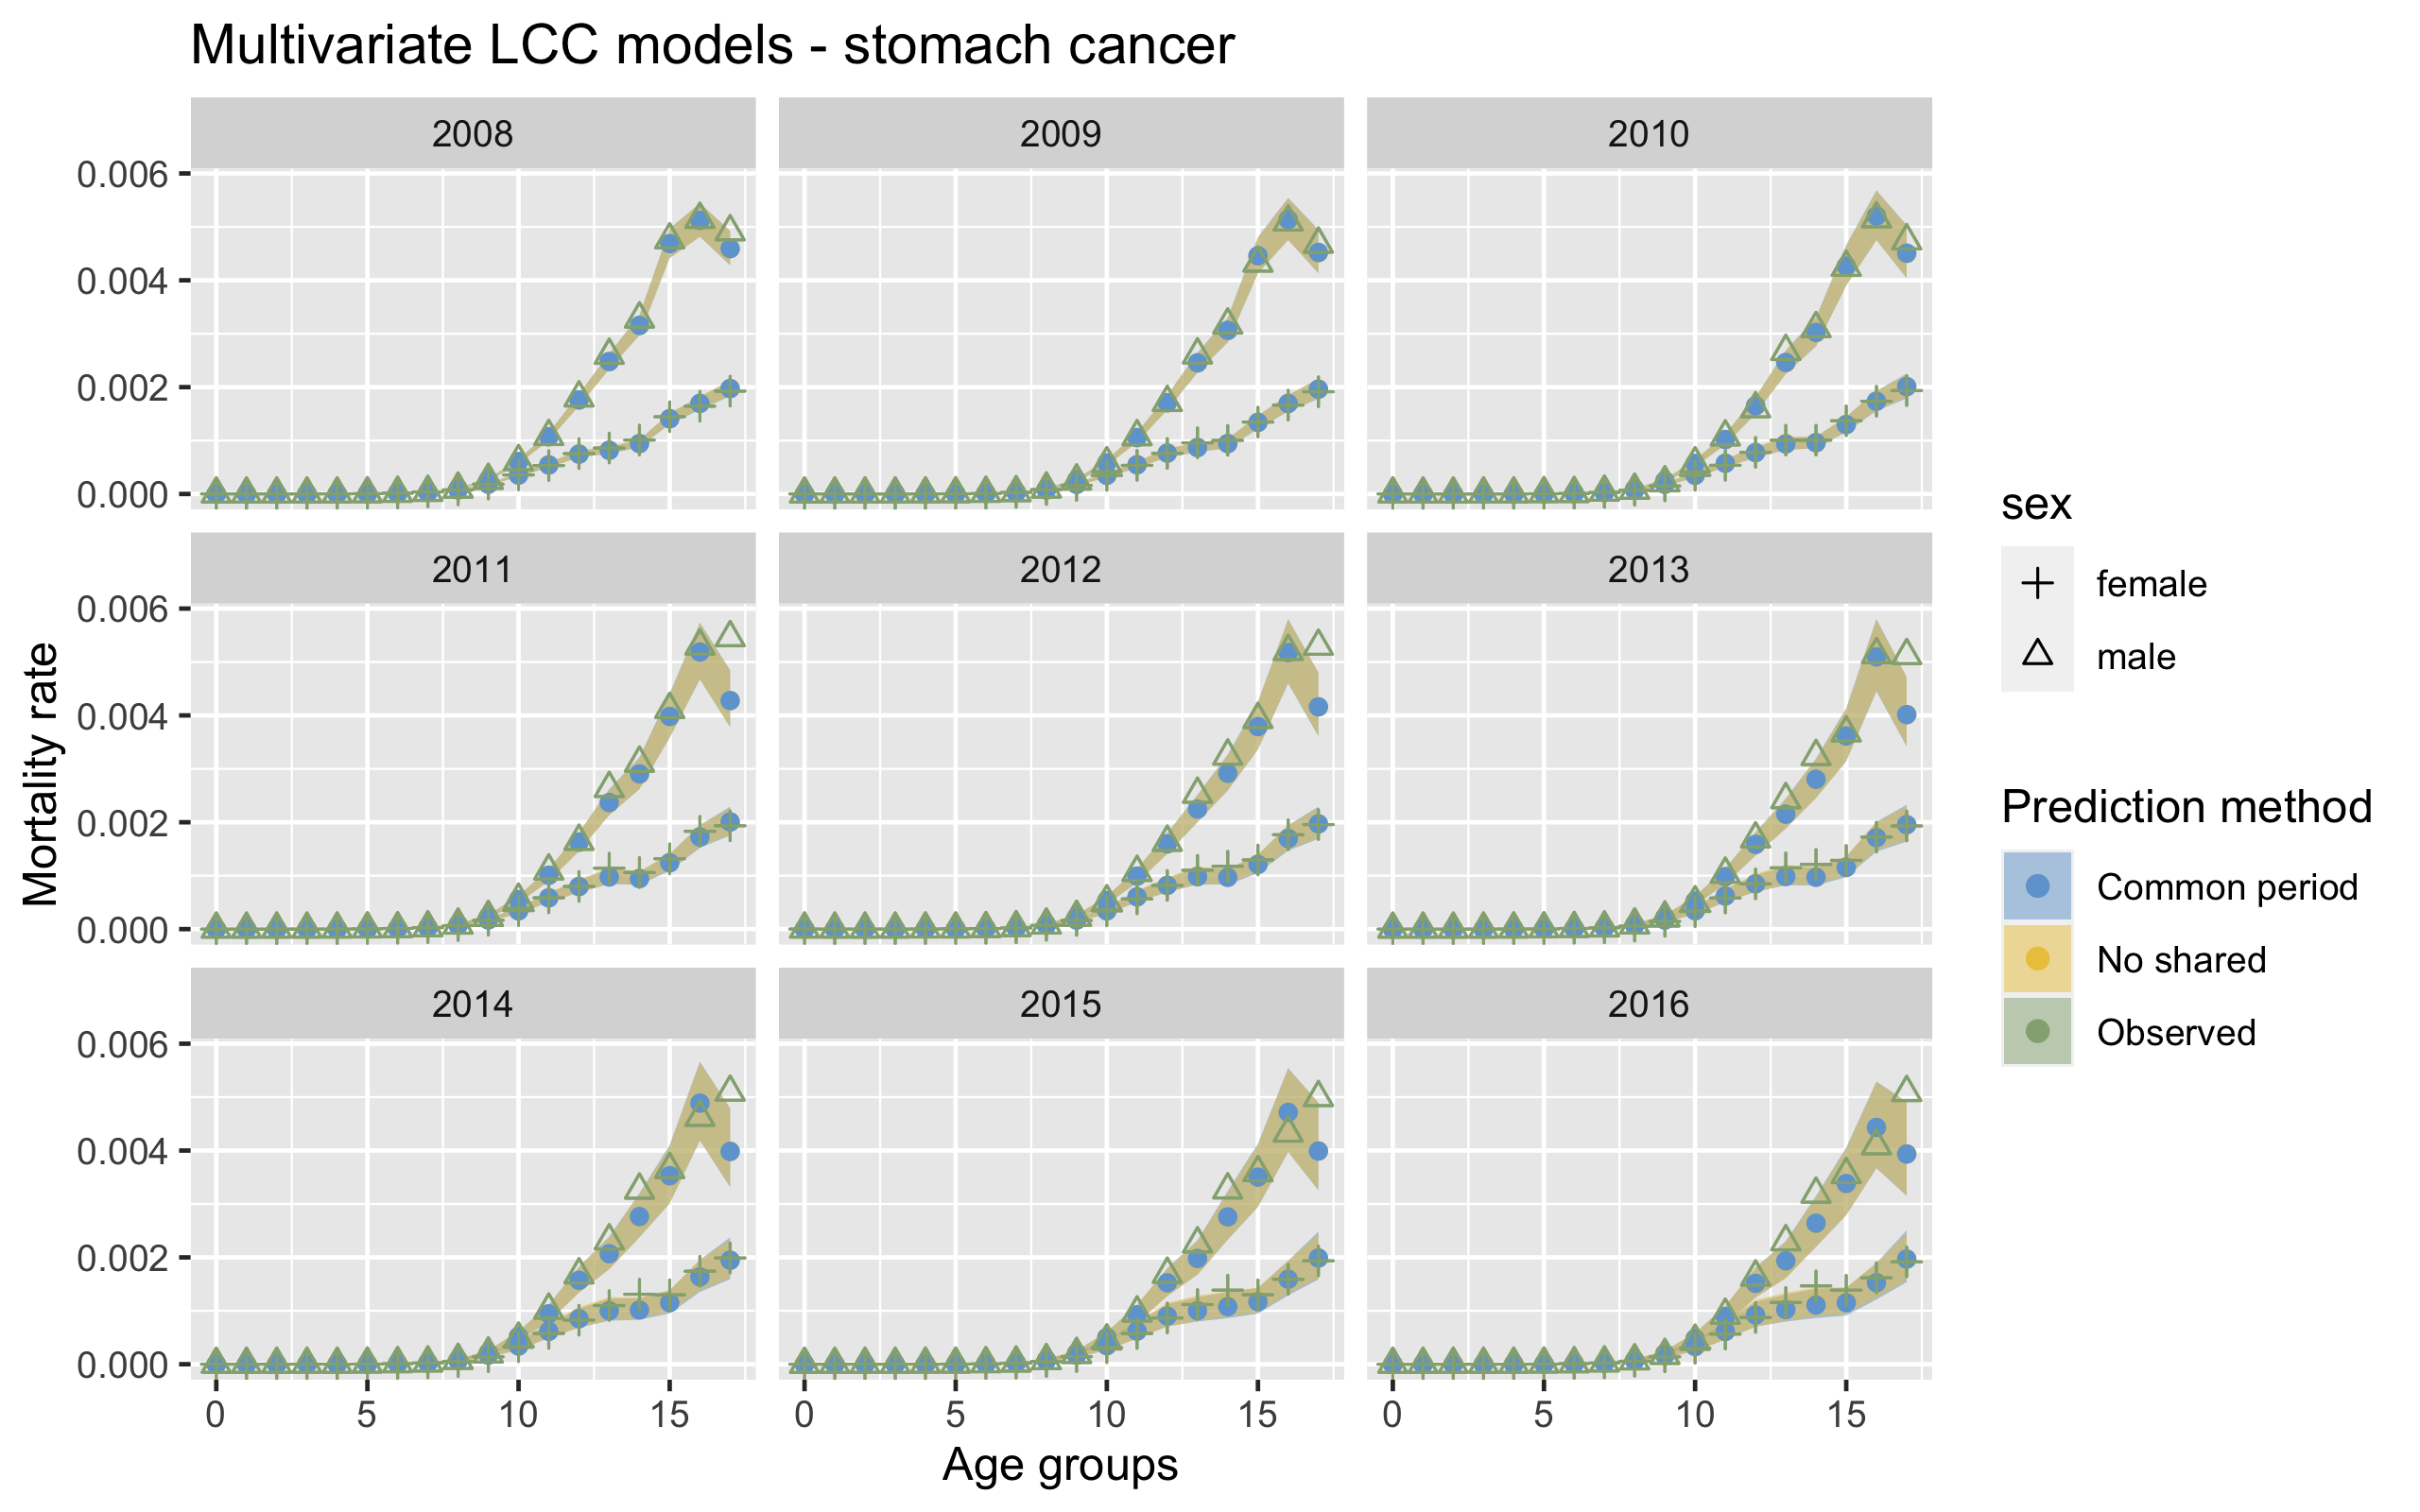
\includegraphics[width=\linewidth]{real-data/real-data-multivariate/Figures/multivariate-LCC-by-age-stomach.png}
%     \end{subfigure}
%     \begin{subfigure}[b]{.45\linewidth}
%         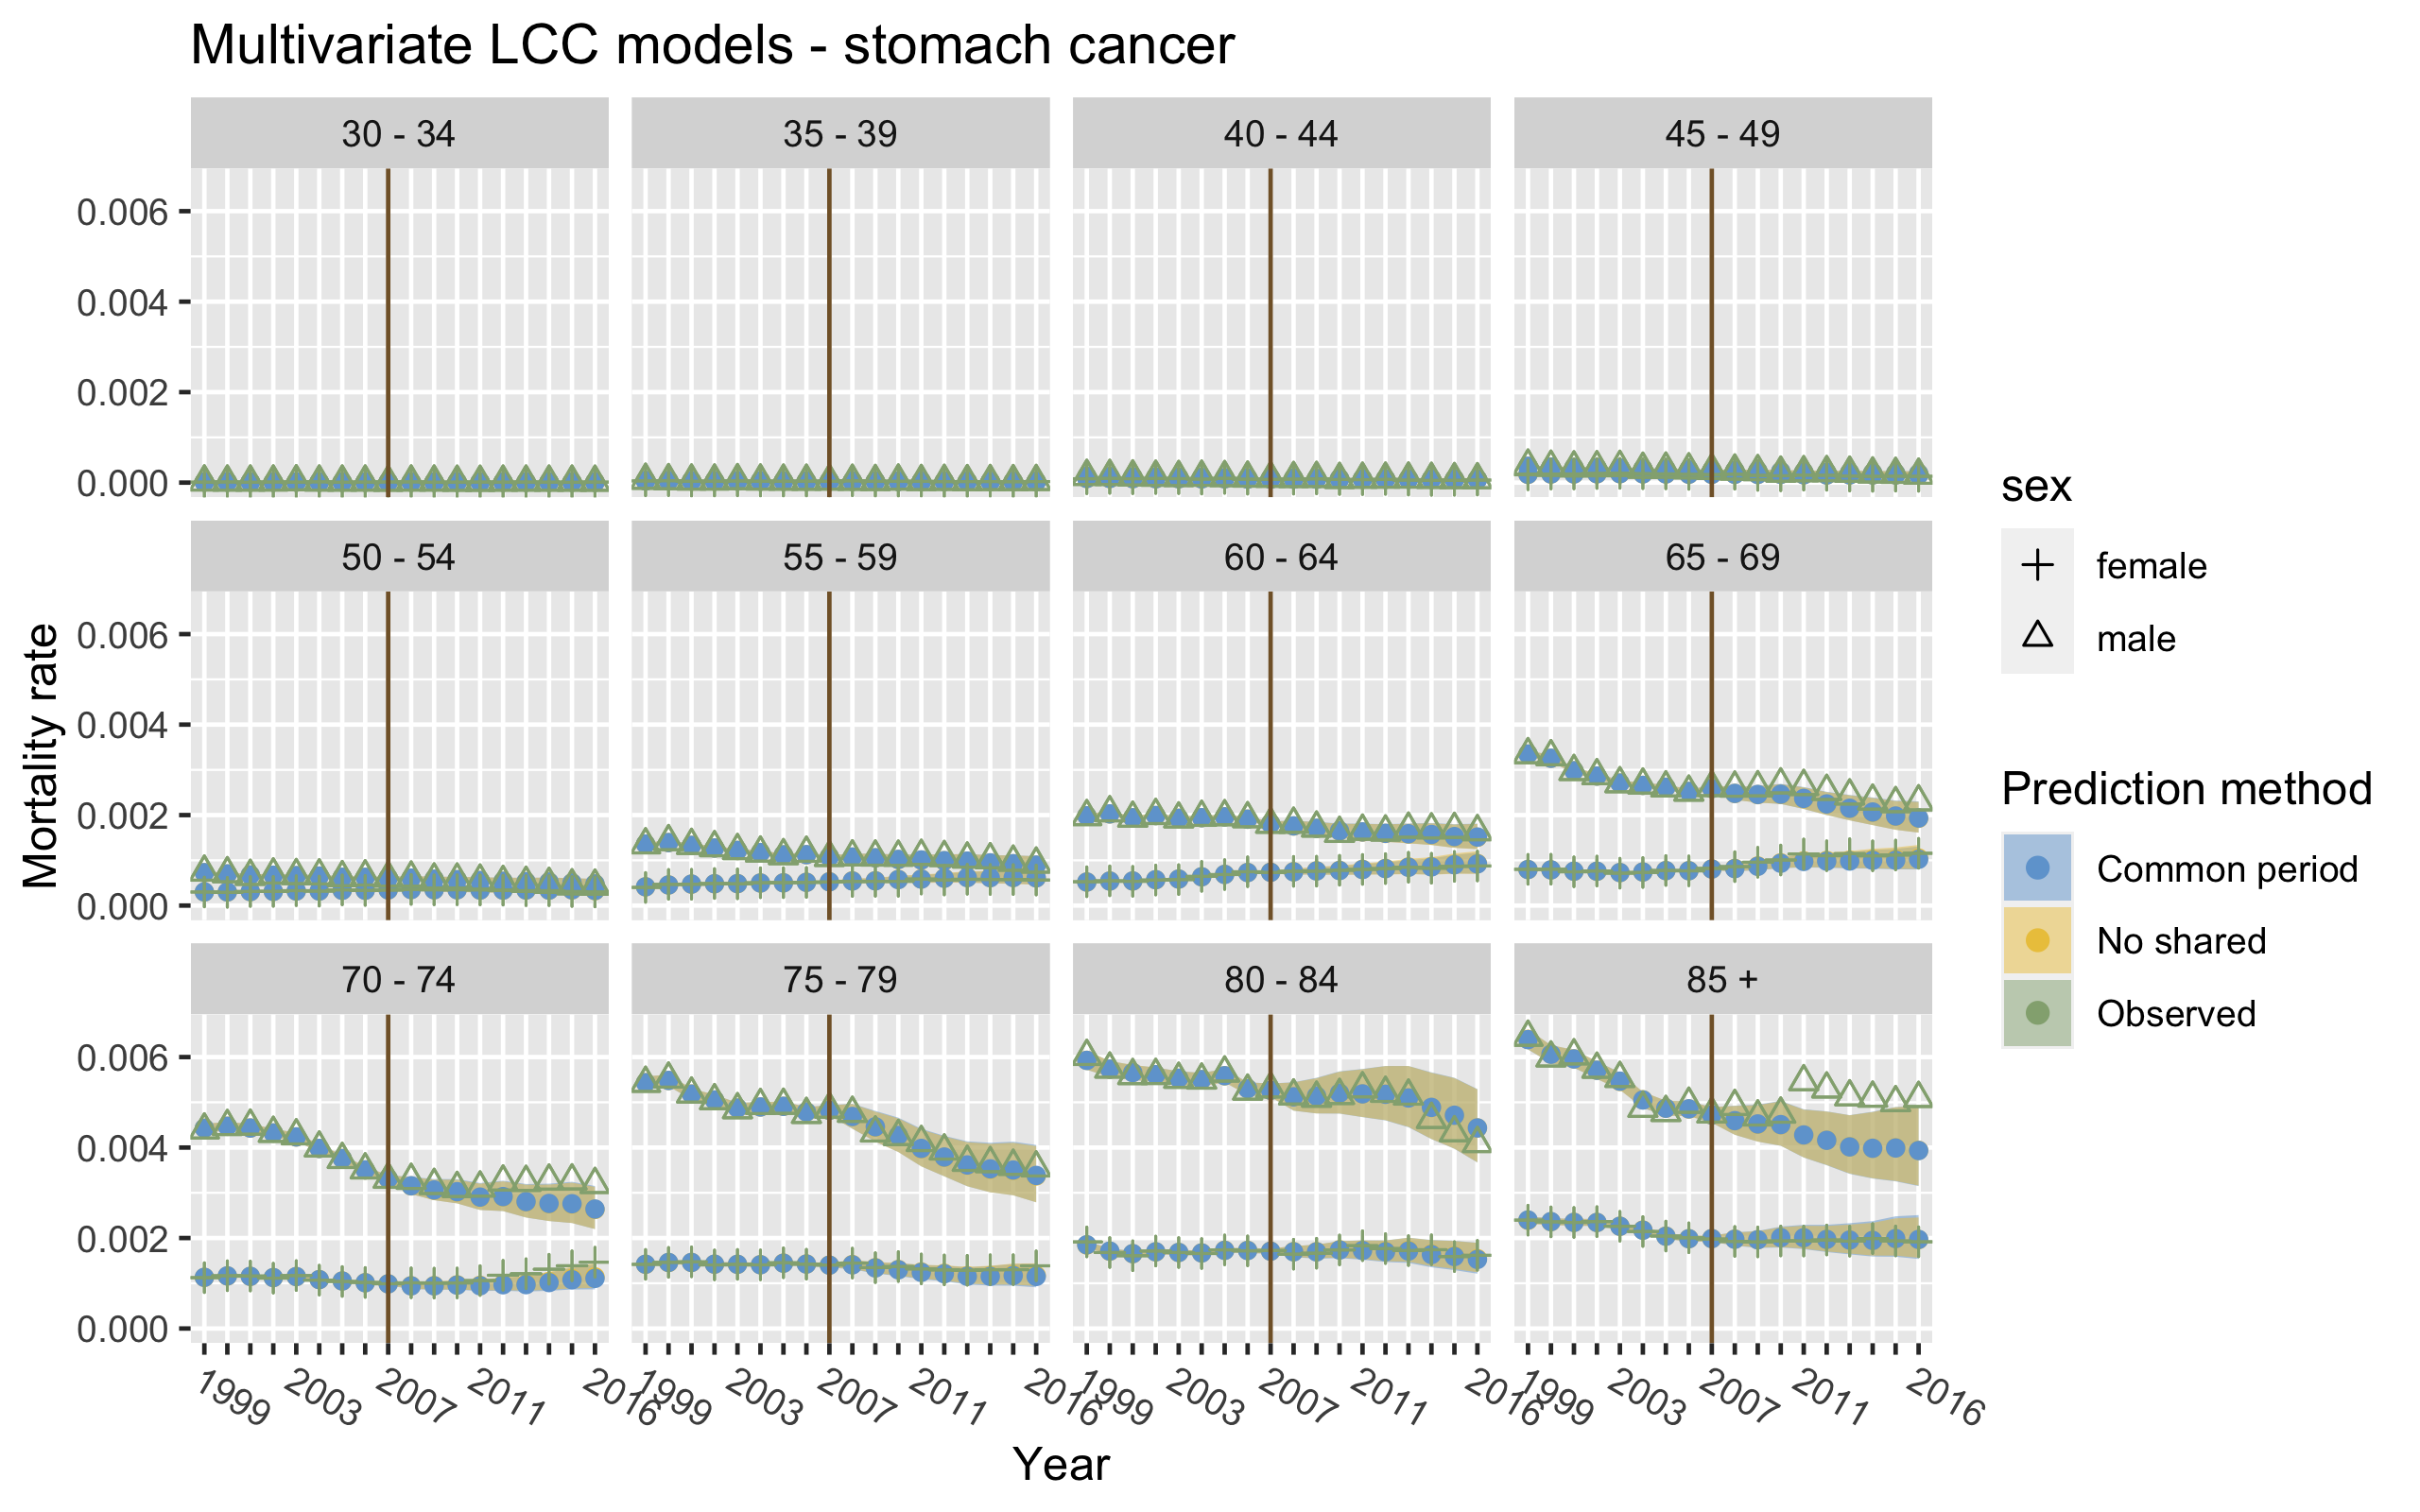
\includegraphics[width=\linewidth]{real-data/real-data-multivariate/Figures/multivariate-LCC-by-period-stomach.png}
%     \end{subfigure}
%     \caption{The two best LCC models - by age (left) and period (right) for the stomach cancer data set}
%     \label{fig:mv-LCC-stomach}
% \end{figure}

% \begin{figure}[h!]
%     \centering
%     \begin{subfigure}[b]{.45\linewidth}
%         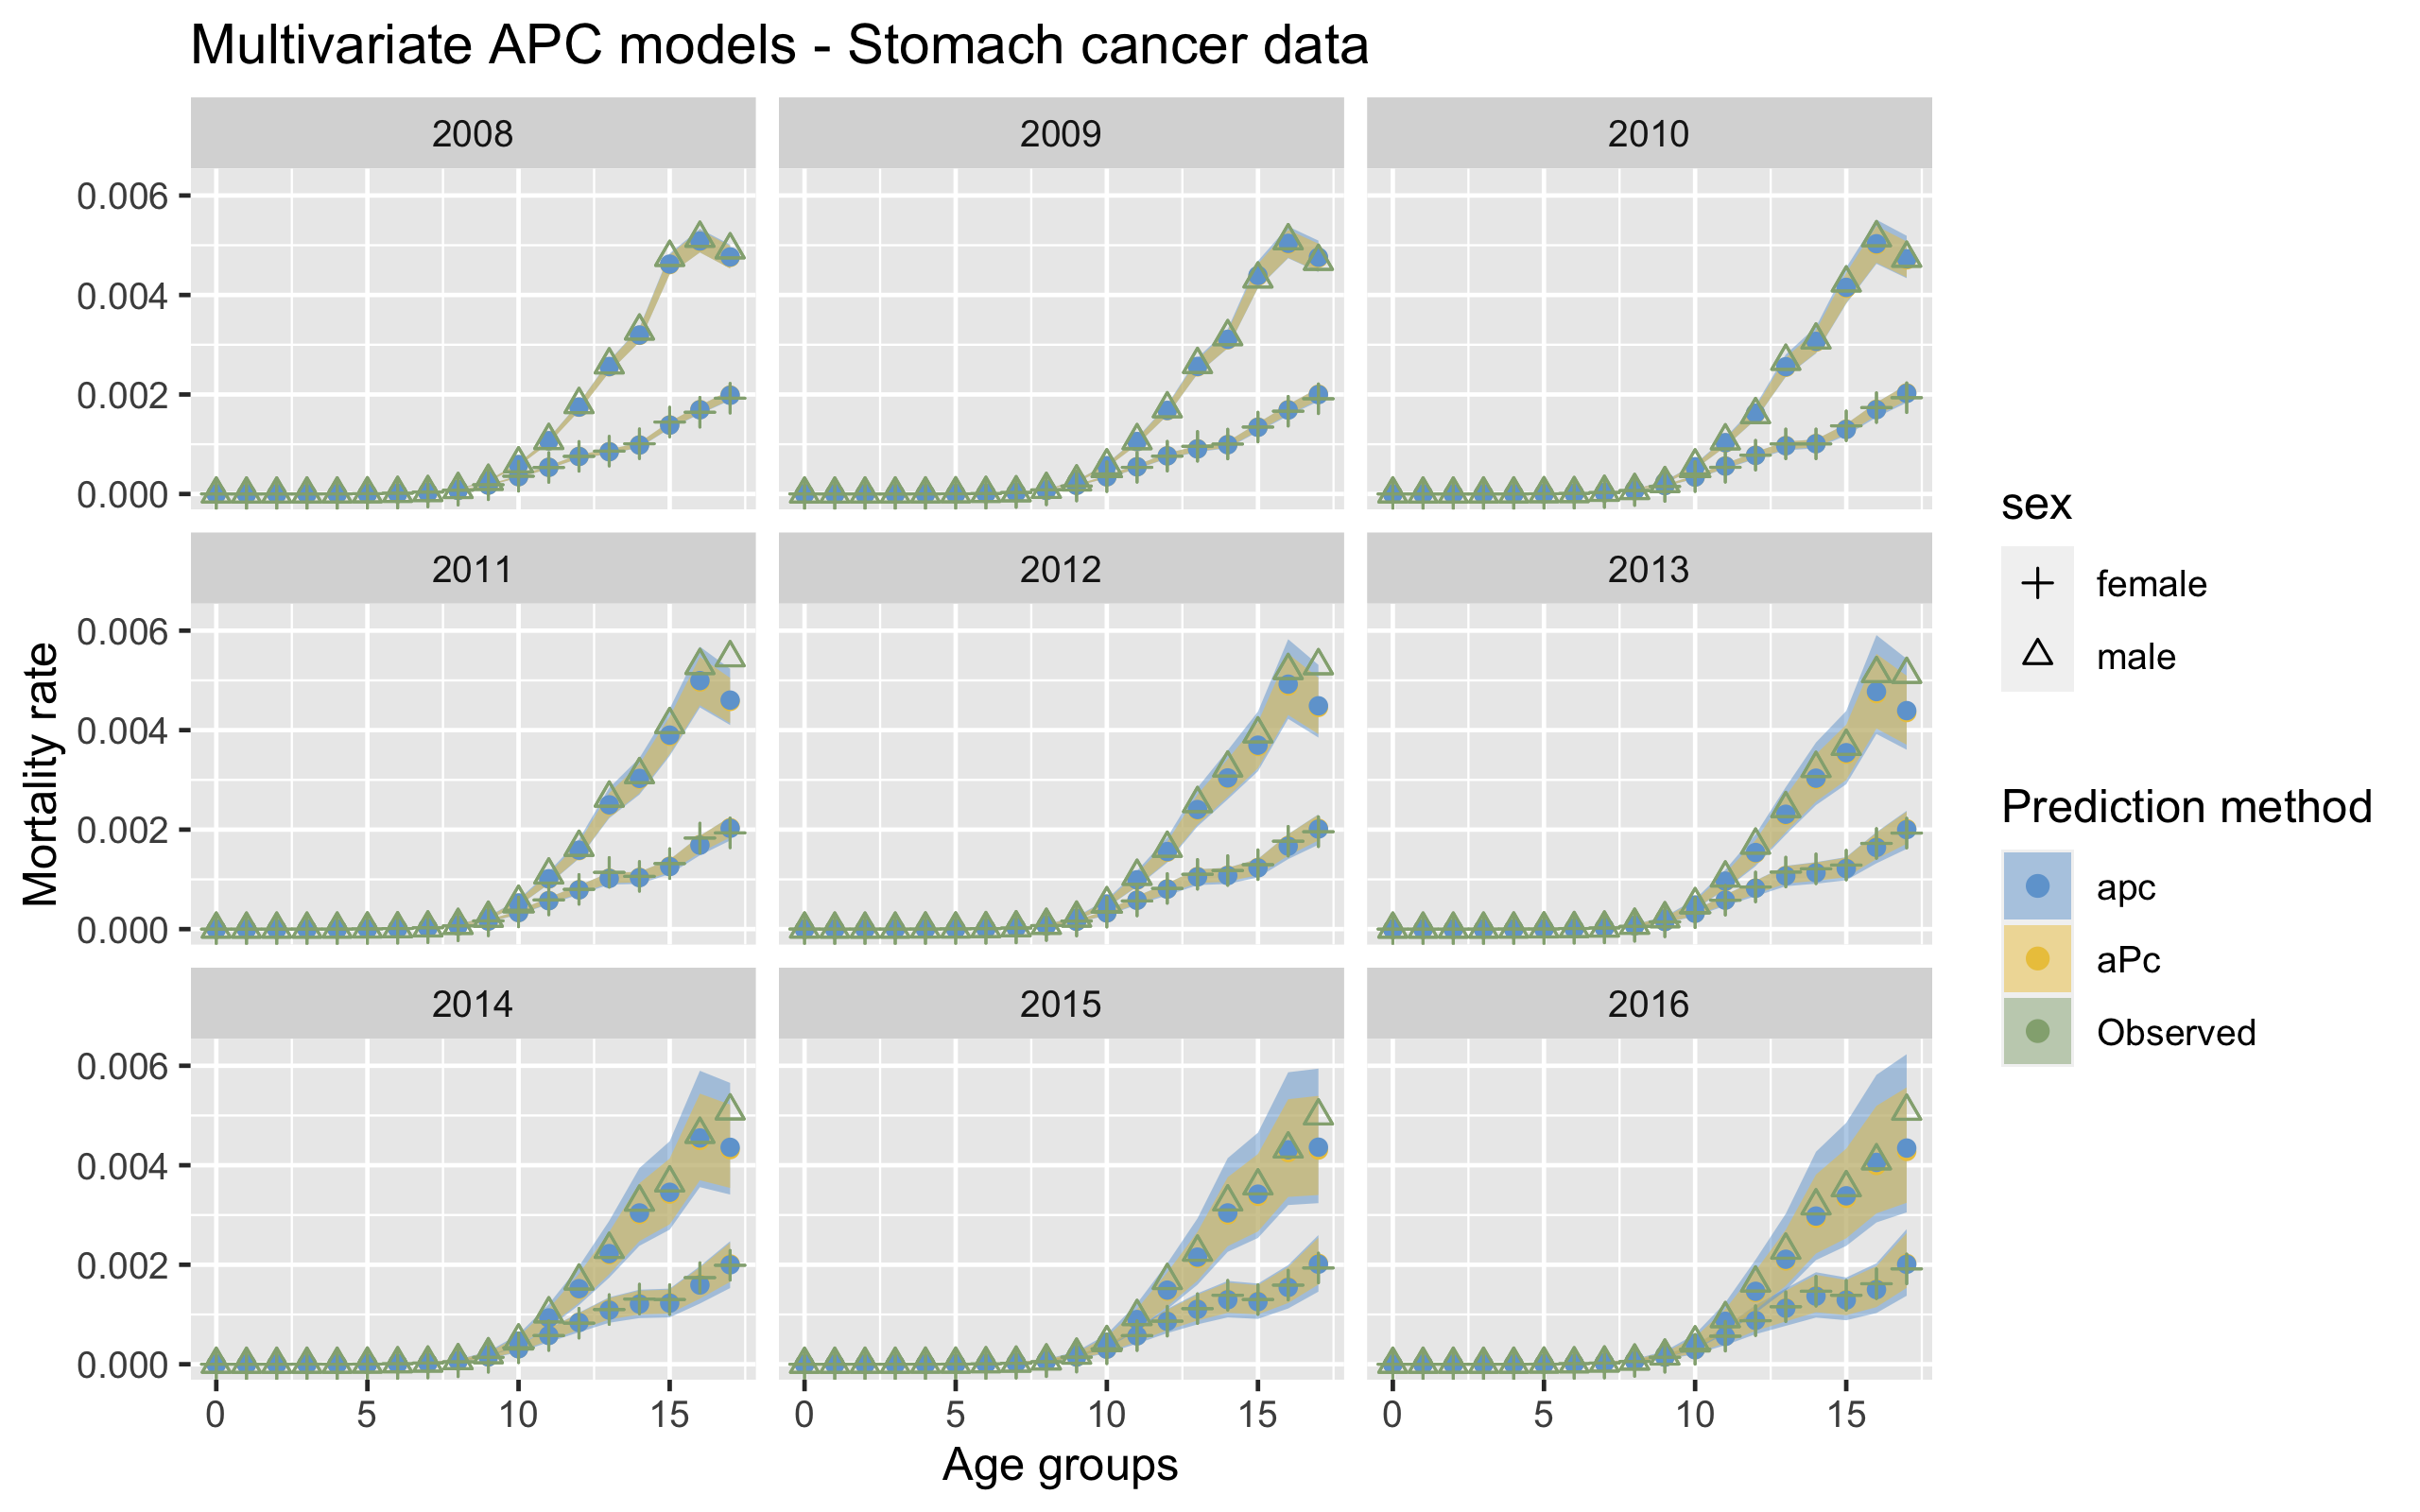
\includegraphics[width=\linewidth]{real-data/real-data-multivariate/Figures/multivariate-APC-by-age-stomach.png}
%     \end{subfigure}
%     \begin{subfigure}[b]{.45\linewidth}
%         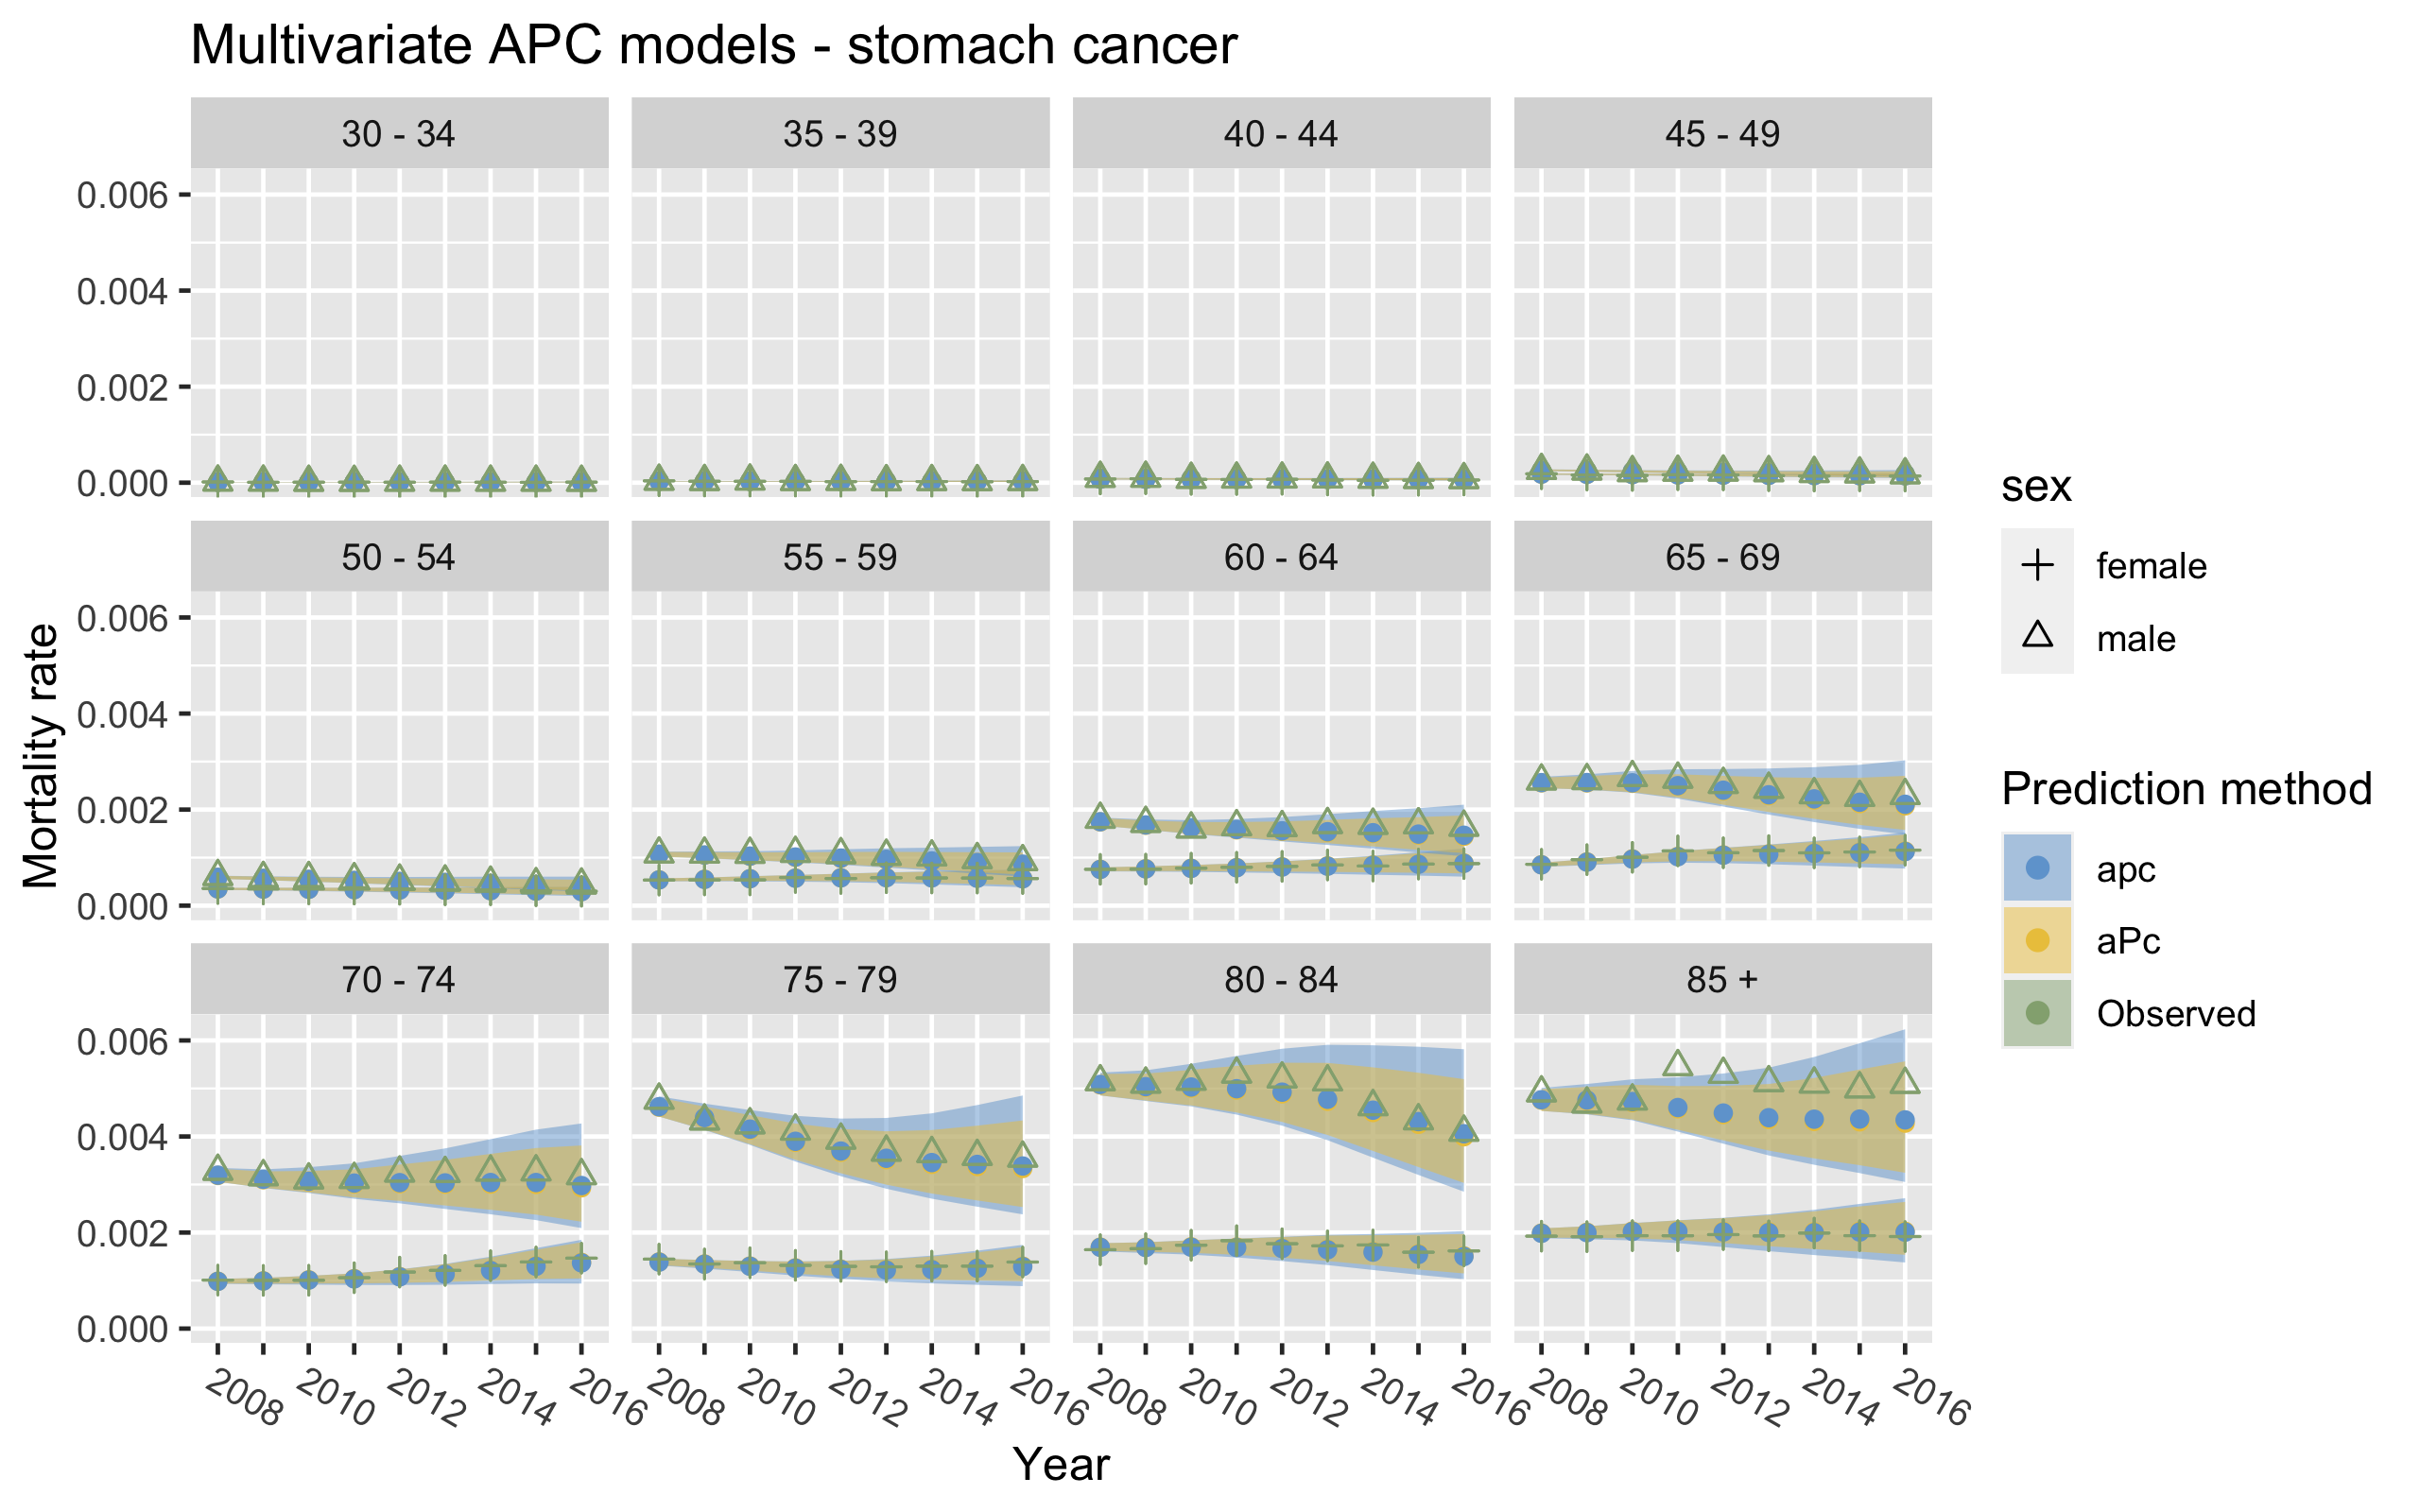
\includegraphics[width=\linewidth]{real-data/real-data-multivariate/Figures/multivariate-APC-by-period-stomach.png}
%     \end{subfigure}
%     \caption{The two best APC models - by age (left) and period (right) for the stomach cancer data set}
%     \label{fig:mv-APC-stomach}
% \end{figure}

\newpar The prediction results from the "Common period"-model and the aPc-model are displayed in Figure \ref{fig:mv-LCC-APC-stomach}. Again, we observe little difference between the APC2 and the LCC-model, other than seemingly wider confidence bounds for the APC2-model. We note that out of the two, the APC2-model has the lowest MDSS. Both models fit the female mortality rates for all ages, for all years quite well. The male mortality rates are also most of the time accurately predicted by both models. The exception is the 85+ age group for the years 2011-2016, and to some degree the 70-74 age group for the same period.

\begin{figure}
    \centering
    \begin{subfigure}[b]{.75\linewidth}
        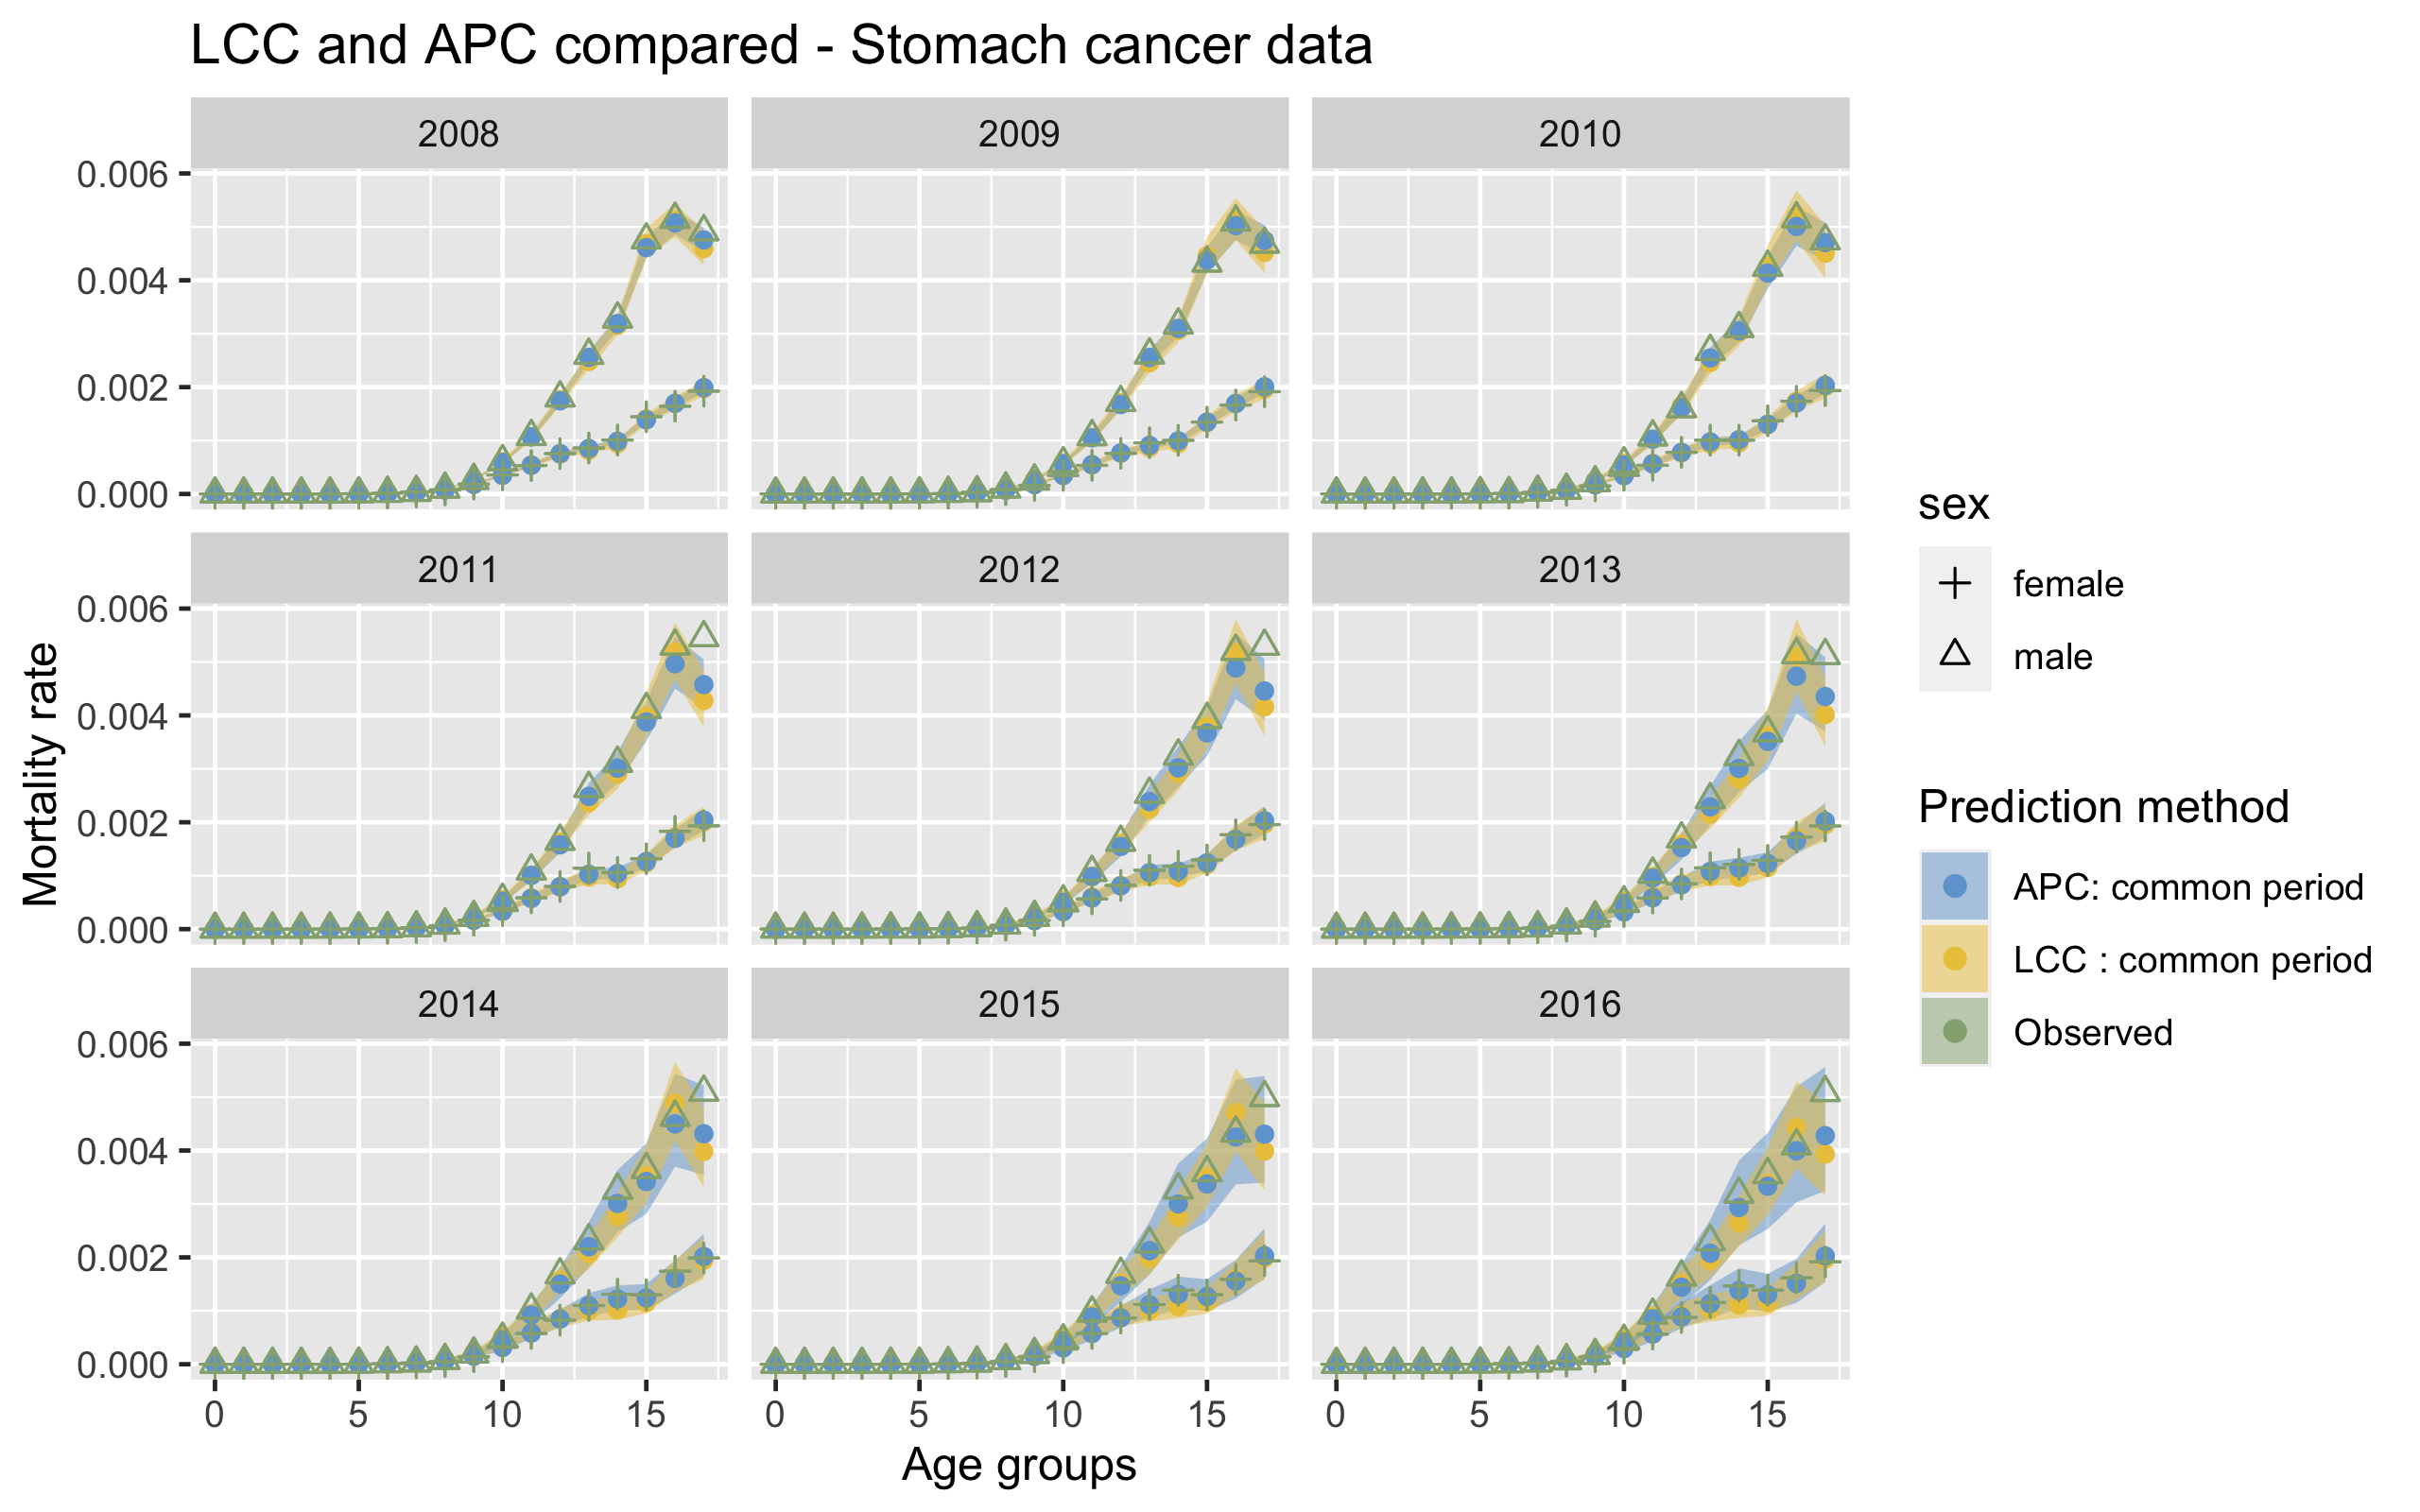
\includegraphics[width=\linewidth]{real-data/real-data-multivariate/Figures/multivariate-comparison-by-age-stomach.png}
        \caption{Age groups along the x-axis}
        \label{fig:mv-LCC-APC-stomach-top}
    \end{subfigure}
    
    \begin{subfigure}[b]{.75\linewidth}
        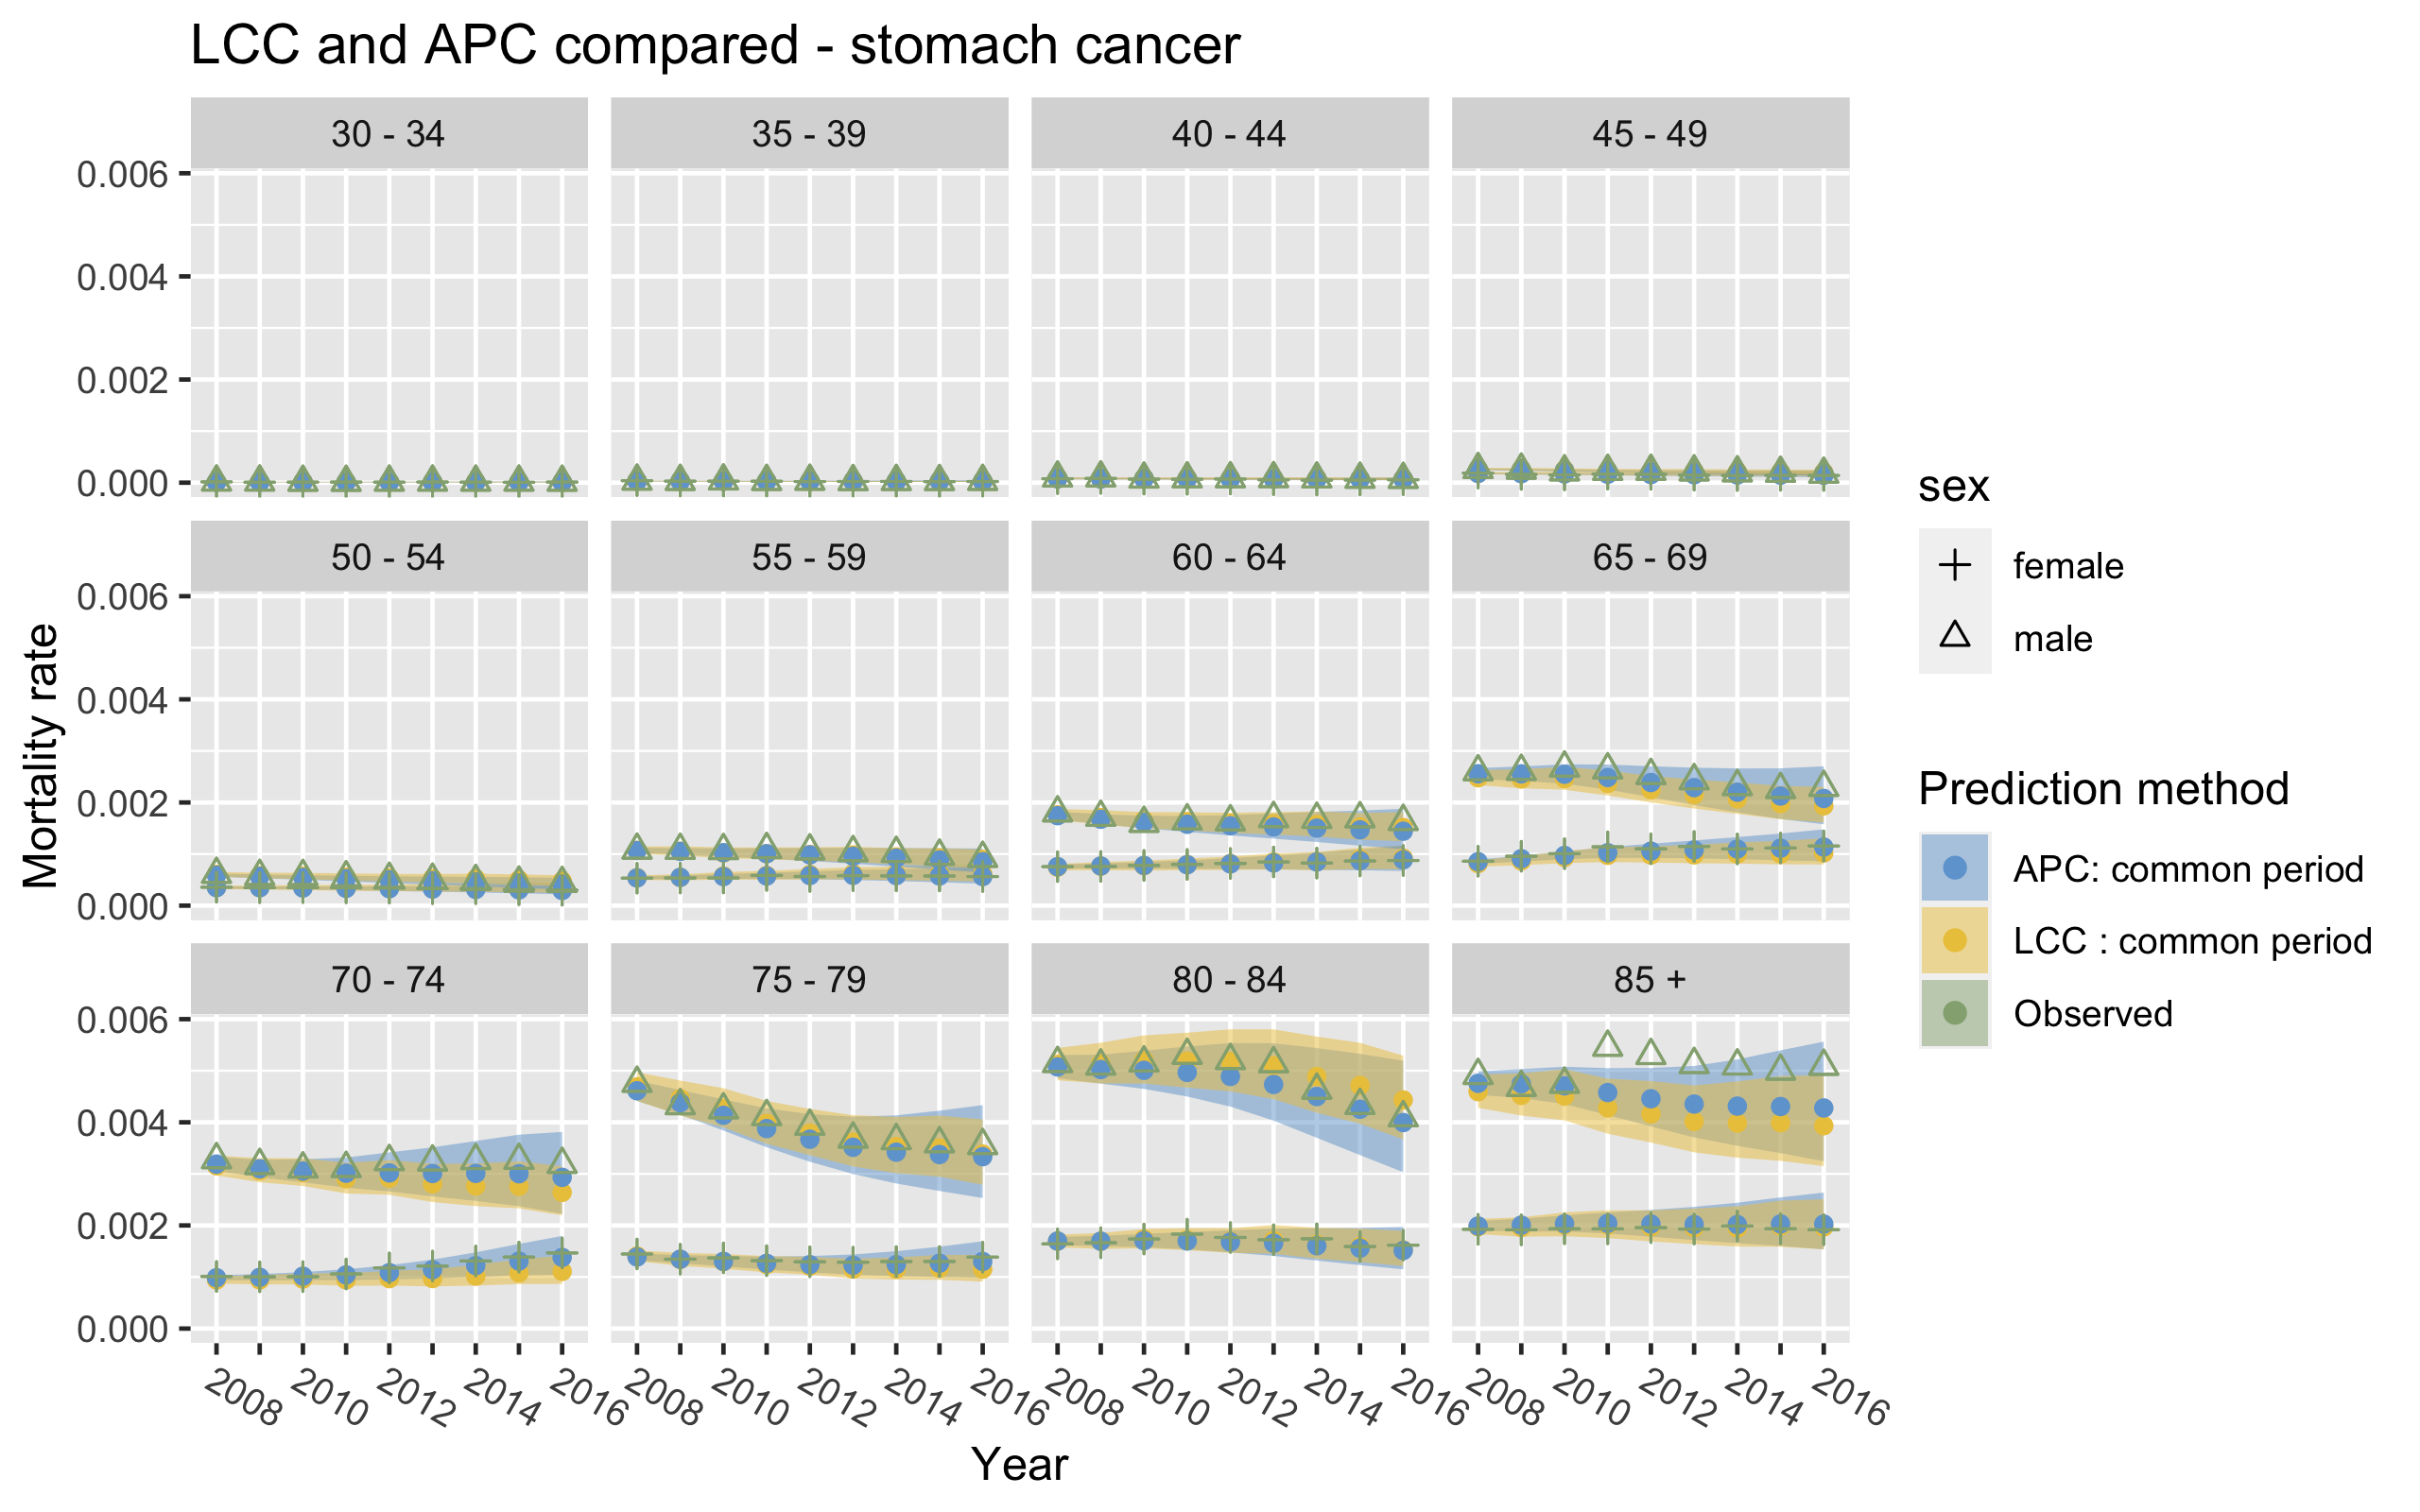
\includegraphics[width=\linewidth]{real-data/real-data-multivariate/Figures/multivariate-comparison-by-period-stomach.png}
        \caption{Year along the x-axis}
        \label{fig:mv-LCC-APC-stomach-bottom}
    \end{subfigure}
    \caption{The mean values and the 95\% confidence bounds of the predicted expected stomach cancer mortality rates produced by inference with the aPc-model and the "Common period"-model on data of German stomach cancer (circles), together with the corresponding observed male mortality rates $Y_{x,y}^{\text{stomach, male}}$ (triangles) and female mortality rates $Y_{x,y}^{\text{stomach, female}}$ (crosses). The layout of the plots is similar to that of Figure \ref{fig:uv-LCC-lung}}
    \label{fig:mv-LCC-APC-stomach}
\end{figure}

\newpar The estimated random effects for the "No common" and the "Common period" LCC-models show similar patterns to those of the same models for lung cancer. Plots of these effects are included in the Appendix, in Figure \ref{fig:effects-LCC-stomach}.

